\documentclass{article}
\usepackage[utf8]{inputenc}

\usepackage{tikz}
\usetikzlibrary{shapes,positioning, arrows.meta, fit, math}

\tikzmath{
\nodeminw = 3;
\nodeminh = 2; 
\nodetextw = 3;
}

\tikzset{
process/.style={draw,
        minimum width=\nodeminw cm,minimum height=\nodeminh cm,align=center,text width=\nodetextw cm,fill=blue!20},
terminal/.style={draw,
    rounded rectangle, 
    minimum width=\nodeminw cm,minimum height=\nodeminh cm,align=center,text width=\nodetextw cm,fill=orange!20},
decision/.style={diamond,draw,aspect=1.95,minimum width=\nodeminw cm,minimum height=\nodeminh cm,align=center,text width=\nodetextw cm,fill=green!20},
io/.style={draw,
    trapezium,
    trapezium left angle = 65,
    trapezium right angle = 115,
    trapezium stretches,minimum width=\nodeminw cm,minimum height=\nodeminh cm,align=center,text width=\nodetextw cm},
point/.style={circle, inner sep=0mm},
}

\begin{document}

\begin{tikzpicture}[x=4cm,y=2cm]

\foreach \i in {2,4,6} {
    \draw (-.75,\i) rectangle (5.75,\i+2);
    \draw (-.75,\i) rectangle (-.5,\i+2);
}
\node[rotate=90,font=\sffamily] at (-.625,7) {Court};
\node[rotate=90,font=\sffamily] at (-.625,5) {FINA};
\node[rotate=90,font=\sffamily] at (-.625,3) {Bidders};

\node[terminal] (request) at (0,7) {Make request\\for sale}; \node[terminal] (suspend) at (2.5,7) {Suspend\\enforcement}; \node[terminal] (adjudication) at (5,7) {Adjudicate decision};
\node[process] (call) at (0,5) {Publish call for participation}; \node[decision] (no_bidders) at (1,5) {No bidders?};  \node[decision] (is_second) at (2.5,5) {Is second auction?}; \node[process] (second_auction) at (4,5) {Start second\\auction}; \node[process] (report) at (5,5) {Send auction\\report};
\node[process] (deposit) at (0,3) {Submit security\\deposit}; \node[process] (bid) at (1,3) {Submit bids};

\node[point] (help1) at (1,5.75) {};
\node[point] (help2) at (4.55,5.75) {};

\node[point] (help3) at (4,4.25) {};
\node[point] (help4) at (0.45,4.25) {};


\begin{scope}[every path/.style={-latex}]
\draw (request) edge (call)
(call) edge node[midway,fill=white,inner sep=2pt] {After at least 60 days} (deposit)
    (deposit) edge (bid)
(bid) edge node[midway,fill=white,inner sep=2pt] {After 10 days} (no_bidders)
(no_bidders) edge node[midway,fill=white,inner sep=2pt] {Yes} (is_second)
(no_bidders) -- (help1)
(help1) -- node[midway,fill=white,inner sep=2pt] {No} (help2)
(help2) edge (report)
(is_second) edge node[midway,fill=white,inner sep=2pt] {Yes} (suspend)
(is_second) edge node[midway,fill=white,inner sep=2pt] {No} (second_auction)
(report) edge (adjudication)
(second_auction) -- (help3)
(help3) -- node[midway,fill=white,inner sep=2pt] {After 1 day} (help4)
(help4) --  (call)
;
\end{scope}

\end{tikzpicture}

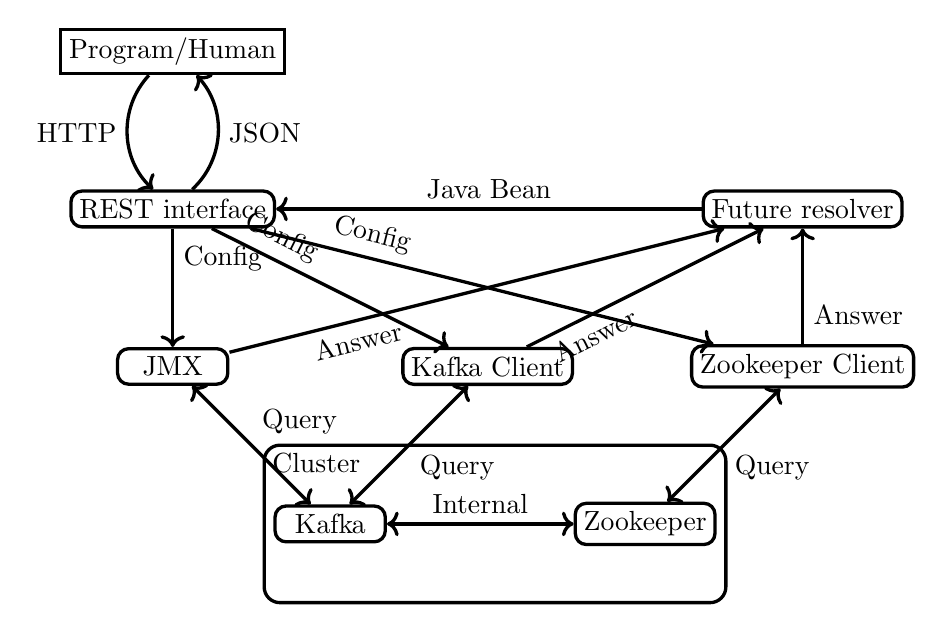
\begin{tikzpicture}[ % has a lot of options; consult the pgf manual
bend angle=45,
long_square/.style={rectangle, draw=black, fill=white, very thick, inner sep=3pt, minimum width=14mm},
rounded_square/.style={rectangle, rounded corners, draw=black, fill=white, very thick, inner sep=3pt, minimum width=14mm},
empty_circle/.style={rectangle, rounded corners=2mm, draw=black, fill=white, very thick, minimum size=4mm},
point/.style={circle, inner sep=0mm},
fit_square/.style={rectangle, rounded corners=2mm, draw=black, very thick, minimum height=20mm},
both_arrow/.style={<->, very thick},
out_arrow/.style={->, very thick},
out_hollow_arrow/.style={-open triangle 90, very thick},
in_arrow/.style={<-, very thick},
dashed_line/.style={loosely dashed, very thick},
above_edge_text/.style={above, midway, sloped}
]

% \node[type](name_of_node)[above/below/right/left/...=of name_of_node]{node_text}
%   edge[<->, bend left/right] node[auto, swap]{edge_text}(out_name_of_node)
% OR
% \node[type](name_of_node)[above/below/right/left/...=of name_of_node]{node_text}

\node[long_square](users) at (0,0) {Program/Human};

\node[rounded_square](REST_interface) at (0,-2) {REST interface};
\node[rounded_square](future_resolver) at (8,-2) {Future resolver};

\node[rounded_square](jmx) at (0,-4) {JMX};
\node[rounded_square](kafka_client) at (4,-4) {Kafka Client};
\node[rounded_square](zookeeper_client) at (8,-4) {Zookeeper Client};

\node[rounded_square](kafka) at (2,-6) {Kafka};
\node[rounded_square](zookeeper) at (6,-6) {Zookeeper};



\node [fit_square, fit=(kafka) (zookeeper)] (cluster) {};
\node [anchor=north west] at (cluster.north west) {Cluster};

% \draw[->](name_of_node.direction) -- (name_of_node.direction)
% OR
% \draw[->](name_of_node.direction) to [bend right] node[]{edge_text} (name_of_node.direction)
% OR
% \draw[->](name_of_node.direction) .. controls +(up/down/right/left:10mm) and +(up/down/right/left:10mm) .. (name_of_node.direction);

\draw[out_arrow](users) to [bend right] node[auto,swap]{HTTP} (REST_interface);
\draw[out_arrow](REST_interface) to [bend right] node[auto,swap]{JSON} (users);

\draw[out_arrow](REST_interface) to [] node[auto,near start]{Config} (jmx);
\draw[out_arrow](REST_interface) to [] node[auto,near start,sloped]{Config} (kafka_client);
\draw[out_arrow](REST_interface) to [] node[auto,near start,sloped]{Config} (zookeeper_client);

\draw[out_arrow](future_resolver) to [] node[auto,swap]{Java Bean} (REST_interface);

\draw[out_arrow](jmx) to [] node[auto,swap,near start,sloped]{Answer} (future_resolver);
\draw[out_arrow](kafka_client) to [] node[auto,swap,near start,sloped]{Answer} (future_resolver);
\draw[out_arrow](zookeeper_client) to [] node[auto,swap,near start]{Answer} (future_resolver);

\draw[both_arrow](jmx) to [] node[auto]{Query} (kafka);
\draw[both_arrow](kafka_client) to [] node[auto]{Query} (kafka);
\draw[both_arrow](zookeeper_client) to [] node[auto]{Query} (zookeeper);

\draw[both_arrow](kafka) to [] node[auto]{Internal} (zookeeper);

\end{tikzpicture}

\end{document}
